\documentclass[letterpaper]{article}
\usepackage[utf8]{inputenc}
\usepackage[T1]{fontenc}
\usepackage[activeacute,english]{babel}
\usepackage[vmargin=4cm,tmargin=3cm,hmargin=2cm,letterpaper]{geometry}%
\usepackage{helvet}
\usepackage{amsmath,amsfonts,amssymb}
\usepackage{graphicx}
\usepackage{color}
\usepackage{xcolor}
\usepackage{verbatim}
\usepackage{tabls}
\usepackage{lastpage}
\usepackage{fancyhdr}
\usepackage{url}
\usepackage{listings}
\usepackage{tikz}
\usepackage{pgf}
\usepackage{pgffor}
\usepgfmodule{plot}
\usepackage{wrapfig}
\usepackage{ifpdf}
\usepackage{amssymb}
\usepackage{pifont}
\usepackage{epstopdf}
\usepackage{graphicx} % Allows including images
\usepackage{booktabs} % Allows the use of \toprule, \midrule and \bottomrule in tables
\usepackage{tikz}
\usetikzlibrary{arrows,decorations,snakes,backgrounds,fit,calc,through,scopes,positioning,automata,chains,er,fadings,calendar,matrix,mindmap,folding,patterns,petri,plothandlers,plotmarks,shadows,shapes,shapes.arrows,topaths,trees}

\lstset{% general command to set parameter(s)
%   basicstyle=\small,
  % print whole listing small
%   keywordstyle=\color{black}\bfseries\underbar,
  % underlined bold black keywords
%   identifierstyle=,
  % nothing happens
%   commentstyle=\color{white}, % white comments
%   stringstyle=\ttfamily,
  % typewriter type for strings
  showstringspaces=false}
  % no special string spaces

\pagestyle{fancy}
\color{black}
\fancyhead{}
\renewcommand{\headrule}{\hrule\vspace*{0.5mm}\rule{\linewidth}{0.8mm}}
\renewcommand{\familydefault}{\sfdefault}

\graphicspath{{./images/}}
\lhead{
\includegraphics[width=2cm]{logoucr.png}}
\rhead{
\includegraphics[width=3cm]{eie-text-gray-6x3cm.png}}
\chead{UNIVERSIDAD DE COSTA RICA\\FACULTAD DE INGENIERÍA\\ESCUELA DE INGENIERÍA ELÉCTRICA\\\textbf{ESTRUCTURAS ABSTRACTAS DE DATOS Y\\ ALGORITMOS PARA INGENIERÍA}\\IE-0217\\I CICLO 2014\\PROPUESTA DEL PROYECTO DE ESTRUCTURAS DE DATOS}

\lfoot{}%
\cfoot{}%
%\cfoot{\thepage\ de \pageref{LastPage}}%
\rfoot{}%

%%%%%%%%%%%%%%%%%%%%%%%%%%%%%%%%%%%%%%%%%%%%%%%%%%%%%%%%%%%%%%%%%%%%%%%%%%%%%%%%%%%%%%%%%%%%%%%%%%%%%%%%%%%%%%%
\newcommand{\uic}{blue} %user-input color
%%%%%%%%%%%%%%%%%%%%%%%%%%%%%%%%%%%%%%%%%%%%%%%%%%%%%%%%%%%%%%%%%%%%%%%%%%%%%%%%%%%%%%%%%%%%%%%%%%%%%%%%%%%%%%%%%%
\newcommand{\uim}{\_\_} %user-input marker
%%%%%%%%%%%%%%%%%%%%%%%%%%%%%%%%%%%%%%%%%%%%%%%%%%%%%%%%%%%%%%%%%%%%%%%%%%%%%%%%%%%%%%%%%%%%%%%%%%%%%%%%%%%%%%%%%%
\newcommand{\userinput}[1]{\textcolor{\uic}{\uim#1\uim}}


%%%%%%%%%%%%%%%%%%%%%%%%%%%%%%%%%%%%%%%%%%%%%%%%%%%%%%%%%%%%%%%%%%%%%%%%%%%%%%%%%%%%%%%%%%%%%%%%%%%%%%%%%%%%%%%%%%
\begin{document}\vspace*{2cm}
%%%%%%%%%%%%%%%%%%%%%%%%%%%%%%%%%%%%%%%%%%%%%%%%%%%%%%%%%%%%%%%%%%%%%%%%%%%%%%%%%%%%%%%%%%%%%%%%%%%%%%%%%%%%%%%%%%

%%%%%%%%%%%%%%%%%%%%%%%%%%%%%%%%%%%%%%%%%%%%%%%%%%%%%%%%%%%%%%%%%%%%%%%%%%%%%%%%%%%%%%%%%%%%%%%%%%%%%%%%%%%%%%%%%%
\begin{center}
\Huge
\textbf{Data Structures Implementations for K-Da Library}
\vspace*{1cm}
\end{center}

\noindent
\small\baselineskip=14pt
\textbf{Estudiantes:} \\
\text{David Pérez Bolaños - B04769}\\
\text{Andrey Pérez Salazar - B25084}\\
\text{Andrés Sánchez López - B26214}\\


\begin{figure}[ht]
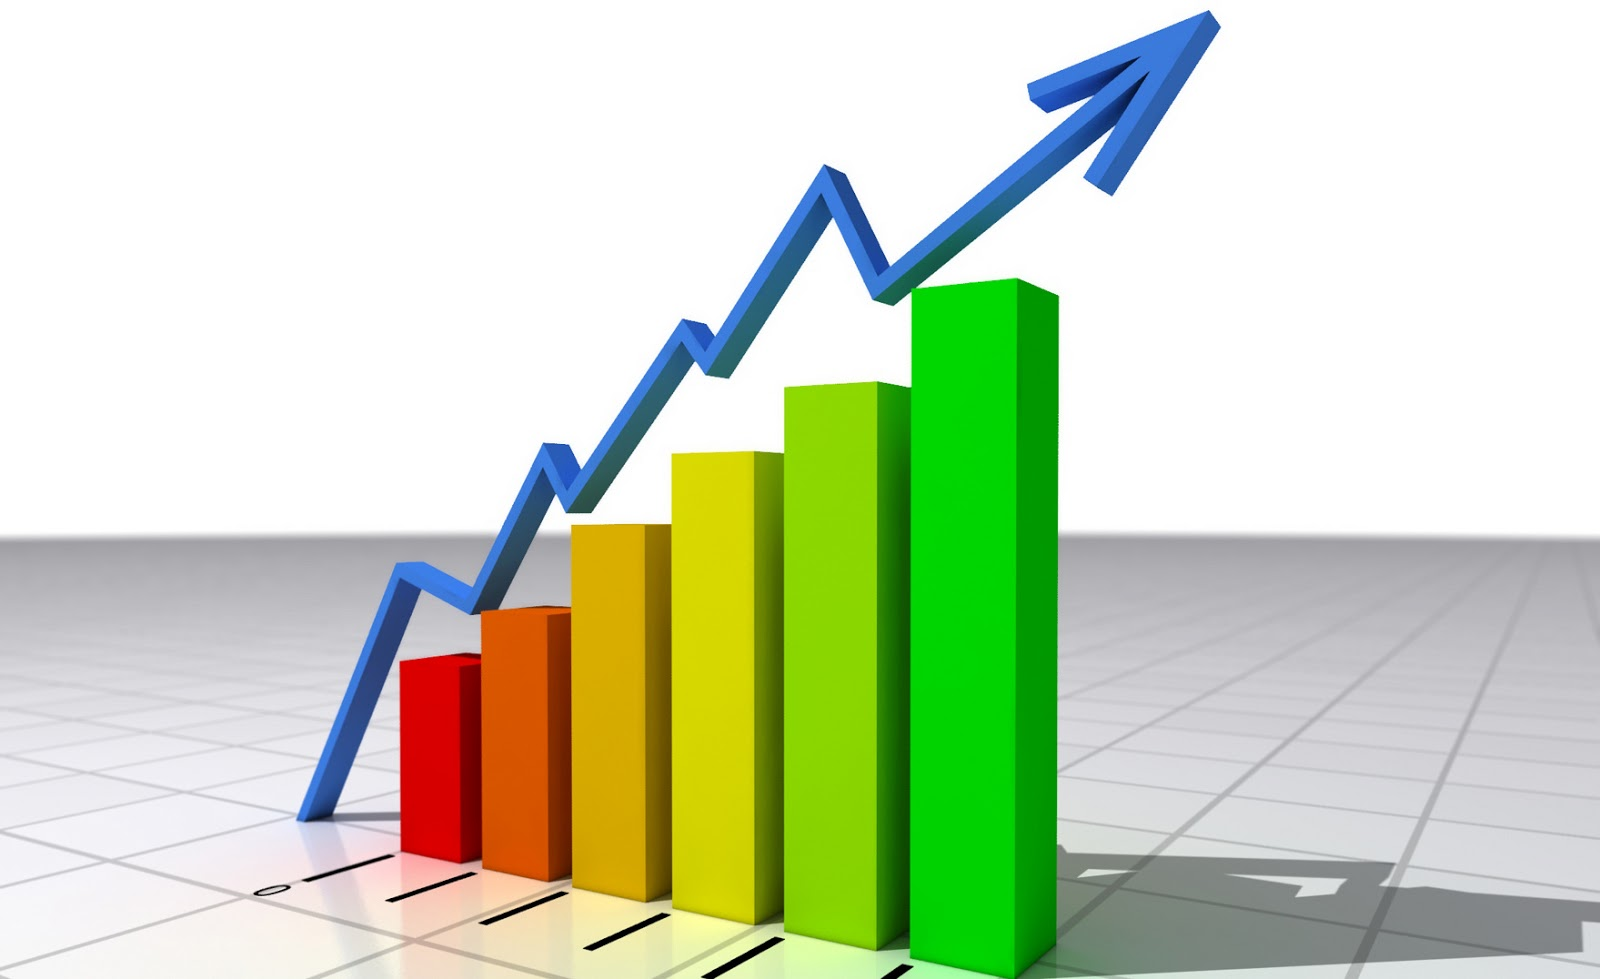
\includegraphics[width=1\linewidth]{ese.jpg}
\end{figure}


%%%%%%%%%%%%%%%%%%%%%%%%%%%%%%%%%%%%%%%%%%%%%%%%%%%%%%%%%%%%%%%%%%%%%%%%%%%%%%%%%%%%%%%%%%%%%%%%%%%%%%%%%%%%%%%%%%
\section{Introducción}
\hyphenation{fun-cio-na-li-dad}
La creación de librerías en lenguajes de programación ayuda a generar una interfaz bien definida para una cierta funcionalidad en específico, 
estas sirven para separar por módulos un programa, y así generar un código más claro y ordenado.\\

Una librería es un conjunto de funciones para desarrollar software, por lo general no son programas, pero si son utilizadas por los programas 
para poder funcionar de forma correcta; el desarrollo de librerías sirve como apoyo para los programadores a tener más facilidades de implementación 
en sus programas y a contar con más recursos para realizar sus proyectos.\\

En este caso, queremos implementar una librería sobre manipulación y análisis de objetos tridimensionales
en el lenguaje C++.\\

La idea  de esta librería es crear métodos o funciones para la manipulación y representación 
de cualquier objeto real, de manera virtual; esta técnica de pasar de un objeto real a representarlo de manera virtual, se utiliza mucho 
en videojuegos, efectos especiales, medicina, simuladores, entre otros.\\

Para nuestro caso utilizaremos para representar los objetos de manera virtual, la técnica de malla de triángulos en 3D, en dónde primero debemos 
representar por medio de una nube de puntos el objeto y luego formar los triangulos con cada uno de esos puntos; para ello utilizaremos el kinect, 
obteniendo así los datos y luego realizar los algoritmos necesarios para la ejecución de las funciones de comparación de datos, generando así la librería.\\


Una segunda parte del proyecto, consiste en la implementación de algunas estructuras de datos para la manipulación de información obtenida mediante el kinect, de manera que se quiere realizar un análisis implementando algunas de ellas, para así determinar y comparar, qué estructuras son las más eficientes a la hora de manipular esta información.\\

En general, las estructuras de datos implementarán las funciones básicas de acceso o búsqueda de datos, lo cual nos ayudará a tener un manejo más rápido y ordenado de los datos obtenidos por el kinect.

 

%%%%%%%%%%%%%%%%%%%%%%%%%%%%%%%%%%%%%%%%%%%%%%%%%%%%%%%%%%%%%%%%%%%%%%%%%%%%%%%%%%%%%%%%%%%%%%%%%%%%%%%%%%%%%%%%%%
\section{Objetivos}

\subsection{Objetivo General}


El objetivo general consiste en analizar algunas de las diferentes estructuras de datos y su desempeño en términos de eficiencia en la librería K-Da
realizada en el primer proyecto del curso.

\subsection{Objetivos Específicos}

Los objetivos específicos son:\\

\begin{enumerate}
\item Ampliar las funciones de la librería K-Da, de modo que se puedan hacer una mayor cantidad de comparaciones de movimientos.
\item Investigar sobre algunas estructuras de datos que puedan mejorar el rendimiento o eficacia de la informacíón utilizada 
en algoritmos de la librería K-Da.
\item Implementar algunas de las estructuras de datos en la librería K-Da para determinar cuáles dan mejores resultados.
\end{enumerate}

%%%%%%%%%%%%%%%%%%%%%%%%%%%%%%%%%%%%%%%%%%%%%%%%%%%%%%%%%%%%%%%%%%%%%%%%%%%%%%%%%%%%%%%%%%%%%%%%%%%%%%%%%%%%%%%%%%
\section{Clases}


(Aquí va la explicación de los métodos de Sama y David)\\

Seguidamente los métodos comparar\_angulos y comparar\_velocidad son los que finalmente evalúan que tan bueno estuvo el movimiento y se lo indica al usuario, esto lo hace utilizando como base los datos suministrados por las clases y métodos anteriores. Primeramente el método comparar\_angulos lo que hace es tomar el arreglo de unos y ceros proveniente de arreglo\_promedio y sumar todos los datos del arreglo, al ser este un arreglo de puros unos y ceros y de longitud 10, el valor de esta suma debería ser máximo 10 y mínimo cero, por lo tanto se puede hacer una evaluación de que tan bien estuvo el movimiento en base al valor de esta suma, si por ejemplo la suma dió uno, esto quiere decir que solo una decima parte del movimiento lo hizo casi igual o muy parecido al movimiento ``ideal'' por lo tanto el restante 90\% del movimiento lo hizo mal en comparación al movimiento ``ideal'', lo que haría que en general el movimiento haya sido muy malo (para este ejemplo). Si por otro lado la sumatoria dió un valor de 5 esto quiere decir que la mitad del movimiento estuvo bien hecho y la otra mitad no, y así sucesivamente hasta llegar a un valor de la sumatoria de 10, lo cuál significaría evidentemente que el movimiento fue excelente. Seguidamente el método comparar\_velocidad lo que hace es determinar que tan rápido el usuario hace el movimiento en comparación con el movimiento ``ideal'', esto ya que de nada serviría tener un 10 en comparar\_angulos si se hizo el movimiento muy lento, ya que efectivamente el movimiento sería igual pero no sería lo correcto decirle al usuario que estuvo bien su movimiento si dura mucho tiempo en ejecutarlo, este método toma la longitud del arreglo de ángulos de los 2 movimientos y los compara, si hay una diferencia de más de un 10\% se lo indica al usuario, diciendole que fue muy lento si se tuvo un 10\% más o que fue muy rápido si se tuvo un 10\% menos. \\
%%%%%%%%%%%%%%%%%%%%%%%%%%%%%%%%%%%%%%%%%%%%%%%%%%%%%%%%%%%%%%%%%%%%%%%%%%%%%%%%%%%%%%%%%%%%%%%%%%%%%%%%%%%%%%%%%%


\section{Cronograma}

\begin{center}
\begin{tabular}{l l   @{\hspace{1cm}}p{10cm}}
\cline{3-3}

\toprule
\textbf{Semana} & \textbf{Fechas} & \textbf{Actividad} \\
\midrule
1 & 1 a 7 de junio & Estudio de las posibles estructuras de datos a utilizar en el proyecto. \\
2 & 8 al 14 de junio & Implementación de las diferentes estructuras de datos escogidas. \\

3 & 15 al 21 de junio & Análisis de eficiencia de las estructuras de datos escogidas. \\
4 & 22 al 28 de junio & Determinación de la mejor estructura de datos y realización del informe.\\

\bottomrule
\end{tabular}
\end{center}

\section{Referencias}

\begin{enumerate}

\item Richard, J. Computer Science Division. University of California at Berkeley. Triangle. A Two-Dimensional Quality Mesh Generator and 
Delaunay Triangulator. Encontrado el 13 de abril del 2014 en: http://www.cs.cmu.edu/~quake/triangle.html
\item Escenografía Intermedial. Nuevos medios y tecnologías afines a la escena. (15 de mayo del 2012).
Nube de puntos (Point Cloud) con Kinect. Encontrado el 13 de abril del 2014 en: http://escenografiaaumentada.wordpress.com/2012/05/15/148/
\item OPENKINECT. Encontrado el 13 de abril del 2014 en: http://openkinect.org/wiki/Main\_Page
\item Joyanes, L., Sánchez, L. \& Zahonero, I. (2007). Estructuras de datos en C++ (1ra ed.) Madrid: McGraw-Hill / Interamericana de España, S.A.



\end{enumerate}

	
\end{document}

